\documentclass[a4paper,10pt,openright,openbib,twocolumn]{article}
%\usepackage[portuges]{babel}
\usepackage[T1]{fontenc}
\usepackage{ae}
\usepackage[utf8]{inputenc}
\usepackage[pdftex]{graphicx}
\usepackage{url}
\usepackage{listings}
\usepackage{verbatim}
\usepackage{enumerate}
\usepackage[pdftex, bookmarks, colorlinks, linkcolor=black, urlcolor=blue]{hyperref} 
\usepackage[a4paper,left=2.5cm,right=2.5cm,top=3.5cm,bottom=3.5cm]{geometry}
\usepackage{colortbl}
\usepackage[margin=10pt,font=small,labelfont=bf]{caption}
\usepackage{mdwlist}
\usepackage{cleveref}
\usepackage{epsfig}

\usepackage{multicol}
\usepackage{appendix}


\setlength{\parindent}{0cm}
\setlength{\parskip}{2pt}


\begin{document}

\begin{multicols}{2}
\title{Study and Optimization of a Finite Volume Application}
\author{
    Brito, Rui\\
    PG22781\\
    Department of Informatics\\
    University of Minho\\
    ruibrito666@gmail.com
  \and
    Alves, José\\
    PG22765\\
    Department of Informatics\\
    University of Minho\\
    zealves.080@gmail.com
}
\date{}
\maketitle
\end{multicols}

\section{Introduction}

This study presents an analysis of the application conv-diff. This analysis consists in the application profile, the use of several optimization techniques and the discussion of its results.
The program conv-diff calculates the heat transfer through an area using a Finite Volume method.

The objective of this study is to research the different optimization techniques and to achieve an improvement in the program performance.

The study was divided in several stages.
In the first stage a profile of the application was created, identifying its troublesome areas and improving the sequential version.
A second stage dedicated to a shared-memory version using OpenMP.
The third stage to work with a GPU version, using its massive parallelism capabilities, was made in CUDA.
In the fourth stage a naive distributed-memory version was researched using MPI.
Finally in the fifth and final stage one or more methods of the previous stages were to chosen and improved upon. Based in our previous results the progression to an improved OpenMp version seemed obvious and was pursued.

In this extended abstract the contents are presented according to the stages of the project. 
A brief section explaining the case study followed by its profile will be presented first. With this sections providing a thorough analysis of the program, a string foundation is created to develop the optimizations. From here, the optimized versions are presented starting with the sequential version, and followed by the OpenMP and CUDA versions. 
After a brief explanation of the MPI version a more extended section is presented introducing the final optimization. 
A final section for a cocnlusion of the project is also presented.
%Finally a section explaining the results is presented followed by a conclusion of the project.
%Two brief appendix are presented with the methodology, systems specifications and roofline.

\section{Case Study}

The application analyzed for this study is \emph{conv-diff(Convection-Diffusion)}.This application simulates the way heat is transferred in a fluid using the finite-volumes method.To compute the heat diffusion, the surface is represented as a mesh. Being represented by cells and edges, the algorithm will traverse all edges, calculating the contribution of the adjacent cells. This application rests in a Finite Volume Library (FVLib), which handles the structures and some of the logic functions necessary for the problem's solution.

The application's main objective is to compute a vector $\overline{\phi}$ such that $\overline{\phi} \longrightarrow G(\overline{\phi}) = \left(\begin{array}{c}
0\\
0\\
\vdots\end{array}\right)$
This is accomplished in three different stages:
\begin{enumerate}
    \item {We begin with a candidate vector $\phi$}
    \item {For each edge, we compute the flux $F_{ij}$, with $i$ and $j$ being the indexes of the adjacent cells}
    \item {For each cell, we compute $\sum |e_{ij}| F_{ij} - |c_i| f_i$}
\end{enumerate}
Thus: $\phi = \left(\begin{array}{c}
\phi_1\\
\vdots\\
\phi_I
\end{array}\right) \longrightarrow G = \left(\begin{array}{c}
G_1\\
\vdots\\
G_I
\end{array}\right)$


The output can be converted to msh format, which is compatible with gmsh, for following data visualization(\cref{fig:parallel}).

\begin{figure}[!htp]
    \centering
    \begin{minipage}[t]{\columnwidth}
        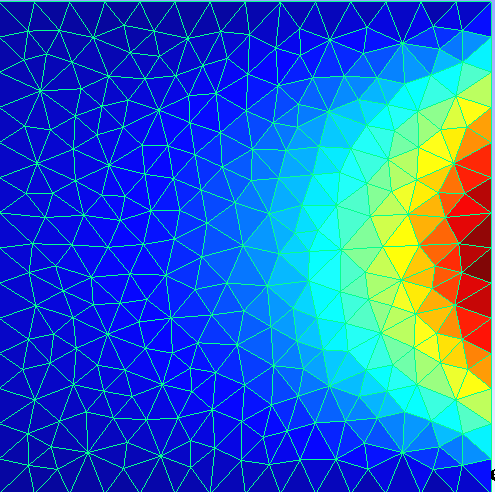
\includegraphics[width=\textwidth]{images/mesh_output.png}
        \caption{Output example.\label{fig:parallel}}
    \end{minipage}
\end{figure}


\section{Profiling}

The program consists in four major parts, reading the initial mesh from a file. Then, using the functions \emph{makeResidual}, which calls the function \emph{makeFlux}, the flux contributions are calculated and the vector phi is built, thus achieving a matrix free implementation. Following this, to calculate the deviation in the results from the previous operations, the function \emph{LUFactorize}. Finally, both the meshes are written to the output files, together with the error between them.
 
After analyzing the application, we conclude that the algorithm has a very high workload in the \emph{LUFactorize} function, comprising of more than 90\% of the execution time.
This is mostly because LUFactorize is a matrix implementation of the algorithm presented in the previous section. While it provides accurate results, it's memory usage, for example, make it unusable for big meshes. As an example, a mesh with more than fifty thousand cells will easily consume more than 10 GB of RAM.

We also conclude that a restructure of the code structures was needed. To improve the locality of data a transformation to Structure of Arrays was also planned.

\section{Sequential Optimization}


After dissecting the code and understanding the problem at hand, we began to notice several implementation errors, these errors, such as reading the same variable repeatedly from a file and long chains of calculation with a heavy division at the end, were easy to spot, and could clearly been avoided. We changed all those trivial aspects of the application, which required minimal effort. That being said, this simple optimizations paid results. The computation time has been greatly reduced, with the aforementioned \emph{LUFactorize} function taking an even more prominent role in our profile.

\section{Shared Memory Parallel Optimization(OpenMP)}

After optimizing the sequential code, we turned our efforts to parallelizing the code. The two loops responsible for the matrix free calculations were ideal candidates. We parallelized both this loops. We had some struggles with data-races in these, but we overcame the problems rather easily. The data-races exist because the mesh is traversed by the edges, however, as we found out, if they are traversed by cell, these data-races no longer exist. Also, the library that was provided includes some iterator style structures. These were also a problem, because, while OpenMP as no problem in parallelizing STL iterators, this doesn't hold for \emph{FVlib}'s iterators. So, we had to convert those to a standard for loop. The code was successfully parallelized, however, results were disappointing, execution time didn't decrease noticeably, hinting at a very memory bound application.
This was also the version that was pursued after the conclusion of the optimization possibilities.

\section{GPU version(CUDA)}

Due to the delay on the restructure of the code, the GPU version was unable to be produced. After several difficulties in forming the kernels and trying to send them to the GPU, we realized that this version was too dependant of the data structures.

\section{Distributed Memory Optimization(MPI)}

The final approach for optimizing the code was a MPI version. This version proved to be a big obstacle, having a high level of communication between processes as well as a high level of barrier synchronization. Some of FVLib's templates were hard to serialize and some balacing problems were also encountered. This versionj proved to be very problematic, causing some error spikes, nullifying the final result.


\section{Conclusion}

This extended abstract serves as a introduction to the study here presented. The initial results from the implementations of optimized versions, sequential and parallel, shows small improvements in the computed time. Future iterations of the solutions increase the improvements.

Through the development of the solutions some problems were presented, such as the mesh being disperse and the structures implemented with extensive use of pointers. This problems delayed the development of solutions. The decision of maintaining the abstraction of the system while favorable in terms of comprehension, proves punishing in terms of performance.

In the future released paper a deep analysis of the results will be made, showing the performance improvements obtained.

\end{document}
